\documentclass[11pt]{article}
\usepackage[margin=0.8in]{geometry}
\usepackage{lmodern,microtype,booktabs,graphicx,amsmath,xcolor,hyperref,xurl}
\hypersetup{colorlinks=true,urlcolor=blue,linkcolor=blue,pdftitle={A traffic filter changes counts but not these spike flags},pdfauthor={James N. Jean IV}}
\setlength{\parindent}{0pt}\setlength{\parskip}{6pt}
\newcommand{\MSourceFiles}{12}
\newcommand{\MSourceBytes}{346249}
\newcommand{\MSourceCells}{4920}
\newcommand{\MProjectedRows}{1800}
\newcommand{\MSourceChecks}{8558}
\newcommand{\MDevChecks}{12991}
\newcommand{\MFinalChecks}{12643}
\newcommand{\MDevOrigins}{372}
\newcommand{\MDevUnknown}{168}
\newcommand{\MFinalOrigins}{360}
\newcommand{\MFinalUnknown}{0}
\newcommand{\MWindow}{150}
\newcommand{\MHistory}{28}
\newcommand{\MThreeNative}{4}
\newcommand{\MThreeFiltered}{4}
\newcommand{\MThreeCleared}{0}
\newcommand{\MThreeAppeared}{0}
\newcommand{\MSixNative}{0}
\newcommand{\MSixFiltered}{0}
\newcommand{\MSixCleared}{0}
\newcommand{\MSixAppeared}{0}
\newcommand{\MNineNative}{0}
\newcommand{\MNineFiltered}{0}
\newcommand{\MNineCleared}{0}
\newcommand{\MNineAppeared}{0}
\newcommand{\MPackageACells}{410}
\newcommand{\MPackageADates}{205}
\newcommand{\MPackageAPaired}{150}
\newcommand{\MPackageBCells}{410}
\newcommand{\MPackageBDates}{205}
\newcommand{\MPackageBPaired}{150}
\newcommand{\MPackageCCells}{410}
\newcommand{\MPackageCDates}{205}
\newcommand{\MPackageCPaired}{150}
\newcommand{\MPackageDCells}{410}
\newcommand{\MPackageDDates}{205}
\newcommand{\MPackageDPaired}{150}
\newcommand{\MPackageECells}{410}
\newcommand{\MPackageEDates}{205}
\newcommand{\MPackageEPaired}{150}
\newcommand{\MPackageFCells}{410}
\newcommand{\MPackageFDates}{205}
\newcommand{\MPackageFPaired}{150}
\newcommand{\MPackageGCells}{410}
\newcommand{\MPackageGDates}{205}
\newcommand{\MPackageGPaired}{150}
\newcommand{\MPackageHCells}{410}
\newcommand{\MPackageHDates}{205}
\newcommand{\MPackageHPaired}{150}
\newcommand{\MPackageICells}{410}
\newcommand{\MPackageIDates}{205}
\newcommand{\MPackageIPaired}{150}
\newcommand{\MPackageJCells}{410}
\newcommand{\MPackageJDates}{205}
\newcommand{\MPackageJPaired}{150}
\newcommand{\MPackageKCells}{410}
\newcommand{\MPackageKDates}{205}
\newcommand{\MPackageKPaired}{150}
\newcommand{\MPackageLCells}{410}
\newcommand{\MPackageLDates}{205}
\newcommand{\MPackageLPaired}{150}
\begin{document}
\begin{center}
{\LARGE\bfseries A traffic filter changes counts\\but not these spike flags}\par
\vspace{8pt}James N. Jean IV\\
Independent research and implementation study\quad 30 October 2026\\
{\small Reproducible research, not peer reviewed}
\end{center}
\section*{Decision brief}
A package owner investigating a download spike needs to know which traffic the counter includes. This study compares a fixed anomaly rule on paired PyPIStats totals and publisher-filtered counts. It tests a processing choice, not whether a package gained users or experienced an incident.

Across \MFinalOrigins{} final package-days from six other packages, filtering changes no flag at any of three predeclared thresholds. The primary threshold emits no flags. At the lower sensitivity threshold, both counter views flag the same four Flask dates.

\begin{center}\begin{tabular}{lrrrr}\toprule
Threshold & Native flags & Filtered flags & Cleared & Appeared\\\midrule
3, sensitivity & \MThreeNative & \MThreeFiltered & \MThreeCleared & \MThreeAppeared\\
6, primary & \MSixNative & \MSixFiltered & \MSixCleared & \MSixAppeared\\
9, sensitivity & \MNineNative & \MNineFiltered & \MNineCleared & \MNineAppeared\\\bottomrule
\end{tabular}\end{center}

\textbf{Recommendation.} Retain the counter definition and inspect both today's count and its historical baseline before treating a spike as a reason to investigate. This sample provides no observed alert reduction. Keep the unchanged result and do not lower a threshold after seeing it to manufacture an improvement.

\textbf{What is usable.} Saved paired aggregates, exact accounting, transparent fixed scores, a missingness ledger and an offline exercise let a reviewer inspect why a flag changed or stayed the same. The teaching examples demonstrate both directions, without claiming they occurred in the measured sample.

\textbf{Limits.} Twelve familiar packages form an authored cohort in one current source vintage. Package-days overlap and share an ecosystem. There are no trusted true-anomaly labels, deployment outcomes or measured analyst time savings. The source filter leaves CI/CD traffic and does not identify users. No scientific-priority, causal, adoption or production-readiness claim follows.
\newpage
\section*{1. Source and fixed cohort}
PyPIStats is hosted by the Python Software Foundation and delivers aggregates from PyPI's public BigQuery download data. PyPI identifies its tables and data as CC BY 4.0. Attribution is PyPI / Python Software Foundation and PyPIStats.org; this study selects fields, creates calendar projections and adds calculations. Our code's MIT license does not replace the source data license.

Before statistics collection, twelve package names were sorted by SHA256 and assigned alternately to development and final groups. Each default overall endpoint supplied both categories in one capture. The snapshot contains \MSourceFiles{} exact private entities, \MSourceBytes{} decoded bytes and \MSourceCells{} source category/date cells. No source request was repeated, redirected or denied.

\begin{center}\small\begin{tabular}{llrrr}\toprule
Package & Assignment & Source cells & Source dates & Paired window\\\midrule
pytest & development & \MPackageACells & \MPackageADates & \MPackageAPaired \\
matplotlib & final & \MPackageBCells & \MPackageBDates & \MPackageBPaired \\
httpx & development & \MPackageCCells & \MPackageCDates & \MPackageCPaired \\
urllib3 & final & \MPackageDCells & \MPackageDDates & \MPackageDPaired \\
numpy & development & \MPackageECells & \MPackageEDates & \MPackageEPaired \\
rich & final & \MPackageFCells & \MPackageFDates & \MPackageFPaired \\
pandas & development & \MPackageGCells & \MPackageGDates & \MPackageGPaired \\
flask & final & \MPackageHCells & \MPackageHDates & \MPackageHPaired \\
scipy & development & \MPackageICells & \MPackageIDates & \MPackageIPaired \\
black & final & \MPackageJCells & \MPackageJDates & \MPackageJPaired \\
click & development & \MPackageKCells & \MPackageKDates & \MPackageKPaired \\
requests & final & \MPackageLCells & \MPackageLDates & \MPackageLPaired \\
\bottomrule\end{tabular}\end{center}

Every package has the full \MWindow{}-date window from 1 June through 28 October 2026, producing \MProjectedRows{} public paired rows. The source responses contain more historical labels than the API documentation's approximate retention description; out-of-window cells stay in the qualification ledger and are never scored. No missing window date was zero-filled.

The collector used an ordinary credential-free HTTPS session, retained exact decoded bytes and safe headers, and spaced twelve GET starts by at least ten seconds. The observed acquisition lasted from 21:55:41 to 21:57:31 UTC on 30 October 2026. It used neither a BigQuery job nor an account, key or paid service. Hashes are locally computed entity identities, not publisher checksums.

Private originals are independently reconstructed through SQLite JSON1 in \MSourceChecks{} conditions. Public fields are aggregate counts, dates, package names and provenance. Raw event logs, IP/client records, package files, credentials and formal-publication manuscripts are excluded.
\newpage
\section*{2. The filter is a measurement choice}
Let $W$ be with\_mirrors and $U$ be without\_mirrors. The categories are nested, so the removed amount is $R=W-U$, not a disjoint second audience. The removed share is $R/W$ only when $W>0$; a zero denominator remains undefined.

\begin{center}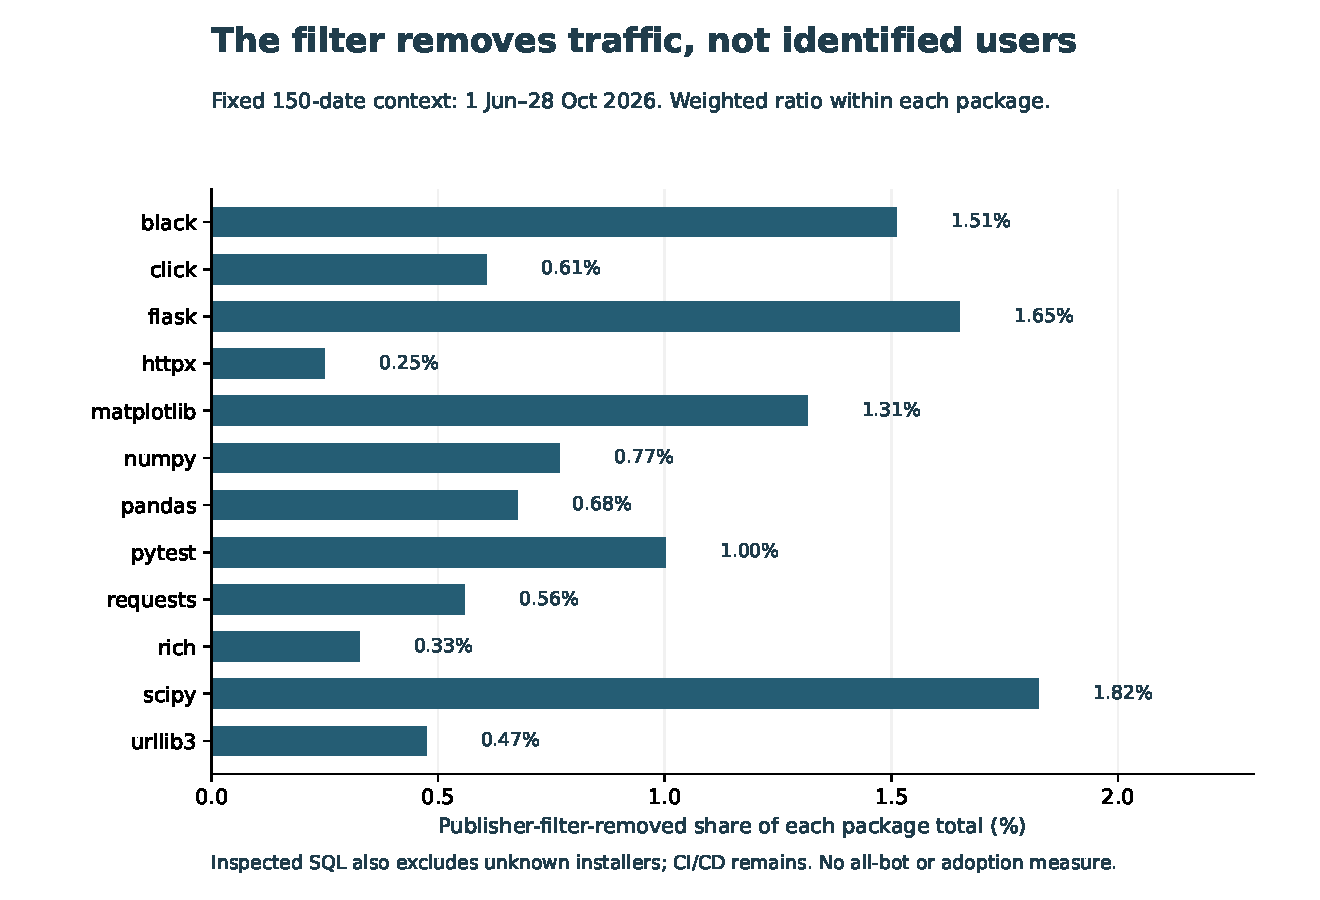
\includegraphics[width=\linewidth]{images/filter_accounting.pdf}\end{center}

The inspected publisher query first restricts Python-version strings (or NULL). Its filtered branch uses installer NOT IN four mirror client names. Under GoogleSQL's NULL semantics, unknown installers also fail that condition. We therefore call the difference \emph{publisher-filter-removed traffic}, rather than an exclusive observed mirror count. The preserved publisher commit and Git blob identities establish inspected code bytes, not which historical deployment generated each daily counter.

The source FAQ says CI/CD remains in the metrics, while requests from end users of mirrors are not reported back. A count reduction cannot identify unique users, remove every form of automation or establish adoption. Each bar is a count-weighted ratio within one package across the fixed window; it is not a ranking of package popularity or value.
\newpage
\section*{3. Fixed scores and unchanged flags}
For current counter $x_t$, calculate the median $m_t$ of $\log(1+x)$ over its own prior \MHistory{} consecutive calendar dates. Let $a_t$ be the median absolute deviation from that median. The authored one-sided score is
\[
 z_t=\frac{\log(1+x_t)-m_t}{\max(a_t,0.1)}, \qquad \text{flag when } z_t>k.
\]
The MAD is unscaled; no Gaussian reference distribution is claimed. The four-week window, 0.1 log-unit floor and $k=3,6,9$ are authored illustrative settings. There is no training fit, tuning or winning threshold.

\begin{center}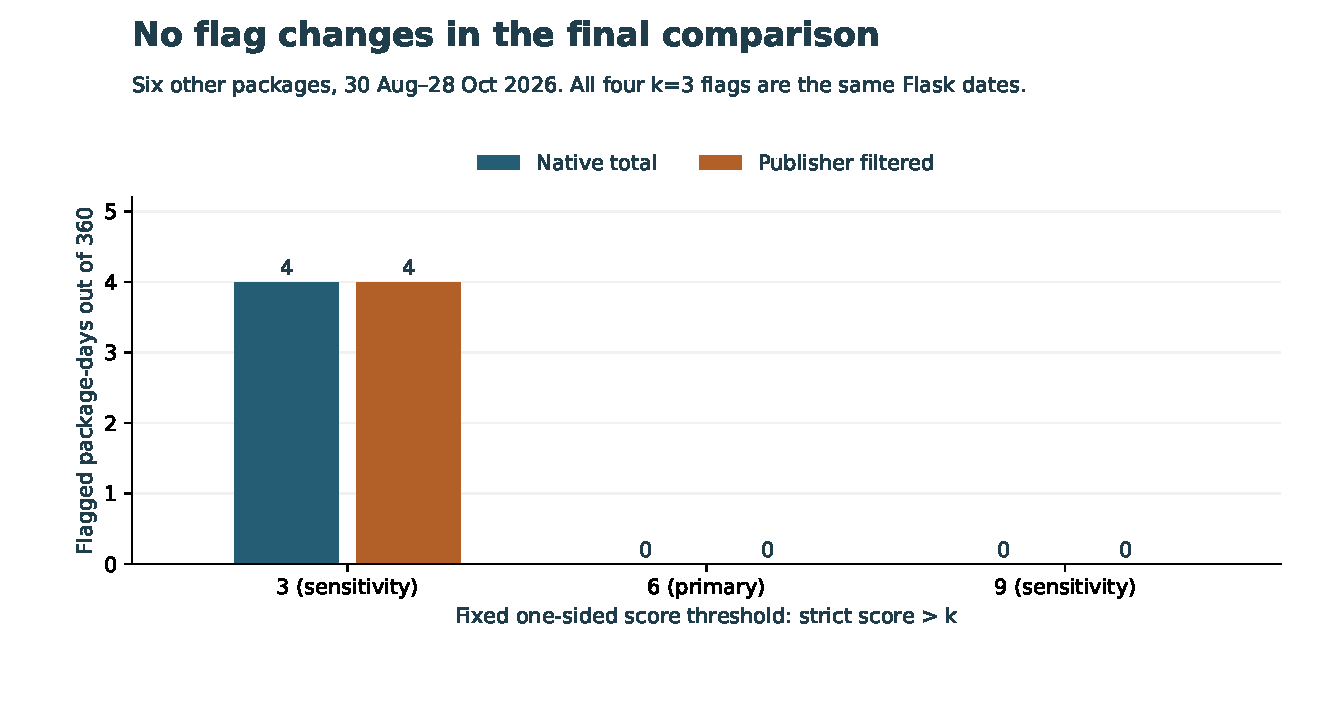
\includegraphics[width=\linewidth]{images/final_flags.pdf}\end{center}

Development uses six assigned packages through 29 August, leaving \MDevOrigins{} scorable origins after \MDevUnknown{} warm-up origins with incomplete history. These are history exclusions, not missing source days. Development has no flags at any setting. A committed manifest of 29 dependencies precedes all final score extraction.

Final evaluation uses the other six packages from 30 August through 28 October, each with its own earlier history. It has \MFinalOrigins{} scorable origins and \MFinalUnknown{} unknown origins. At $k=3$, both views flag Flask on 30 September, 1 October, 27 October and 28 October. No flag clears or appears after filtering. Pooled and equal-package change fractions are both zero. No threshold is adapted after final evaluation.

Source envelopes already include the protected counters before freezing. This is protected analytical evaluation, not blinded collection or an original-vintage forecasting experiment. No false-positive rate, precision, recall or reduction in real workload can be measured without appropriate outcome labels.
\newpage
\section*{4. Both today's count and the baseline matter}
\begin{center}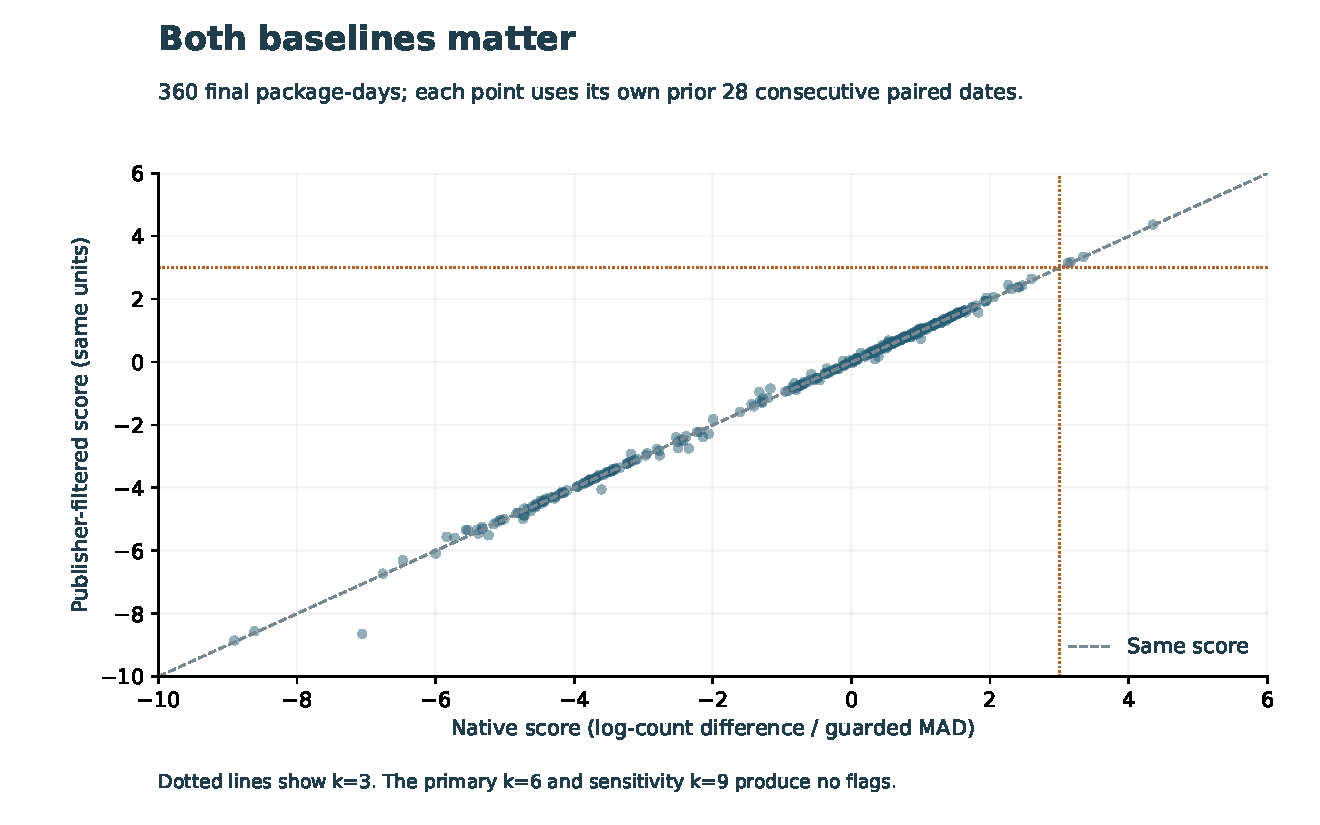
\includegraphics[width=\linewidth]{images/paired_scores.pdf}\end{center}

The main comparison applies the filter to both current counts and history. A secondary view filters only today's count while retaining the native baseline. Because $U_t\leq W_t$ and this baseline is unchanged, its score cannot exceed the native score. It also yields the same four lower-threshold flags and no primary or higher-threshold flags in the final sample.

Filtering both sides can reveal a spike in principle: an authored example has native history 10,000 and filtered history 10, then current counts 1,000 and 100. Although filtering lowers the current count, it reveals an increase relative to the lower filtered baseline. A second authored example removes a current spike while leaving the historical baseline unchanged. These are teaching cases, not discovered incidents.

\begin{verbatim}
python src/review_cli.py examples/removed-current-spike.json
python src/review_cli.py examples/revealed-filtered-spike.json
python src/review_cli.py examples/unknown-short-history.json
\end{verbatim}
The CLI performs no network request or outgoing alert. Missing or short paired histories remain UNKNOWN. Inspect counter provenance and release/deployment context before allocating attention. A broader prospective sample with verified review decisions and incident labels is needed before selecting an operational threshold or claiming benefit.

The original program proposal named direct BigQuery and version-level holdouts. Neither was executed here. The actual delivered scope is paired public aggregate accounting, a separate-package/later-window comparison and a local implementation exercise.
\newpage
\section*{5. Reproducibility and evidence}
Source parsing rejects duplicate JSON object keys and category/date cells, invalid dates, counters that are boolean, noninteger or negative, unknown categories, mismatched identities and $U>W$. All 150 expected dates remain explicit. A scorable origin requires 28 complete consecutive prior paired dates without interpolation or future inputs.

Separate SQLite calendar joins and 80-digit Decimal logarithms, medians and deviations check \MDevChecks{} development and \MFinalChecks{} final conditions. Scores agree within absolute tolerance $10^{-10}$, with exact flags at all three thresholds. Twenty-one fixture methods cover source identity, nested counts, undefined shares, duplicates, missing/short histories, calendar gaps, constant histories, huge counts, strict threshold boundaries, future-count exclusion and redirect bounds. These finite checks do not establish universal software or statistical reliability.

\begin{verbatim}
python -m unittest discover -s tests -v
python src/freeze_proof.py
python src/replay.py --output ../fresh-replay
python src/verify_figures.py
\end{verbatim}
Replay uses a full-history clone, saved aggregates and a fresh external output directory. It preserves source/frozen bytes and performs no source requests. New runtime receipts remain separate from measured originals. Release requires two-runtime isolated replay, source-bound SVG coordinates and hashes, every rendered paper page, a scoped privacy audit and exact remote candidate/main CI, matching tree and annotated tag. Check the selected revision's receipts when reusing the work.

\section*{Primary references and provenance}
\small
Python Software Foundation. \emph{PyPI BigQuery download statistics and data license}. \url{https://docs.pypi.org/api/bigquery/}. CC BY 4.0: \url{https://creativecommons.org/licenses/by/4.0/}.

PyPIStats. \emph{API, hosting information and FAQs}. \url{https://pypistats.org/api/}; \url{https://pypistats.org/about}; \url{https://pypistats.org/faqs}. The FAQ distinguishes nested counters, CI/CD and mirror end-user limits.

PSF. \emph{PyPIStats publisher implementation}. \url{https://github.com/psf/pypistats.org}. Inspected commit: \nolinkurl{2f8271dc7ff1c3fbbbb4f9c09de68f41978cb4ea}; task SQL blob: \nolinkurl{e51531a3202b5304aaeef3d559698c6794c6ad55}; API view blob: \nolinkurl{18bd13b91add14b9f5e5433c0b45ef402510e77d}. The repository's source-revision clarification corrects the historical protocol's tree/commit label while preserving its frozen bytes.

Google Cloud. \emph{GoogleSQL operators, NOT IN and NULL semantics}. \url{https://docs.cloud.google.com/bigquery/docs/reference/standard-sql/operators#in_operator}. The unknown-installer qualification is an inference from this definition and the inspected SQL.

James N. Jean IV. \emph{Download spike context: protocol, counts, checks and implementation exercise}. \url{https://github.com/S3R3Bii/download-spike-context}. Independent study; no new-estimator, priority or deployment claim.
\end{document}
